% the above things have to be place here, or all titles will compromise  --Jordan

\section{Experiment}

\subsection{StyleGAN}
In this section, we will present the result of the style fusion of the source image and target image in Figure \ref{fig:source target image}. The fusion image is present in Figure \ref{fig:stylechange}. According to this result, there are several points that we can discuss.

As shown in Figure \ref{fig:stylechange}, the style interpolation of the reconstructed source image and the reconstructed target image is very successful. We can actually see the hairstyle, faces and background of the reconstructed source image gradually fuse into those of the reconstructed target image with smoothness. The result proves that interpolation of latent code in latent space actually leads to style fusion of image space.

According to Figure \ref{fig:source target image} and \ref{fig:stylechange}, the reconstruction of the source image and the target image is quite a failure. After some discussion, we find out some points that may lead to this undesirable result. These points are listed below:

\subsubsection {Face position problem}
During implementation, we find that the whole reconstructed image will change greatly if we slightly scale the original image. Figure~\ref{fig:face position problem} can fully explain this problem. We divide the four images in Figure~\ref{fig:face position problem} into two groups. The leftmost two pictures are one group, and the rightmost two pictures are another group. Both groups of image contains original image(left one) and reconstructed image(right one). The two images of left part of Figure~\ref{fig:face position problem} is the same as left part of Figure \ref{fig:source target image} and upper left of Figure~\ref{fig:stylechange}. We just cut a little fraction below the neck on the original image Figure \ref{fig:source target image}, the reconstructed image varies a lot (shown in right part of Figure~\ref{fig:face position problem}). 

To be more specific, compared to the reconstructed image that does not cut, the reconstructed image has more hair and wrinkles. The hair and wrinkles, however, have nothing to do with the neck (cut place). We attribute this result to the fact that GAN-based models are inherently very hard to control the generated results.

\subsubsection {Origin goal problem}
The main goal of StyleGAN-based model is to generate diverse results using latent code, while our goal is to reconstruct original image using latent code, which is totally opposite. This might be a potential reason of our bad result.

\subsubsection {Domain gap problem}
The style encoder is trained on FFHQ dataset, which consists mostly of Caucasian and African. Our source and target images are both Asian, which may lead to a domain gap problem.

\subsubsection {Latent code space problem}
Losing information is inevitable when encoding the high dimensional images to low dimension latent vectors. Thus, we will lose considerable information when we perform style encoding. As a result, StyleGAN generator cannot generate images similar to original images.


\begin{figure}[ht]
\centering
    \centering
    \includegraphics[scale=.25]{fig/source_target_pair.png}
    \caption{left: source image, right: target image}
    \label{fig:source target image}
\end{figure}

\begin{figure}[ht]
\centering
    \centering
    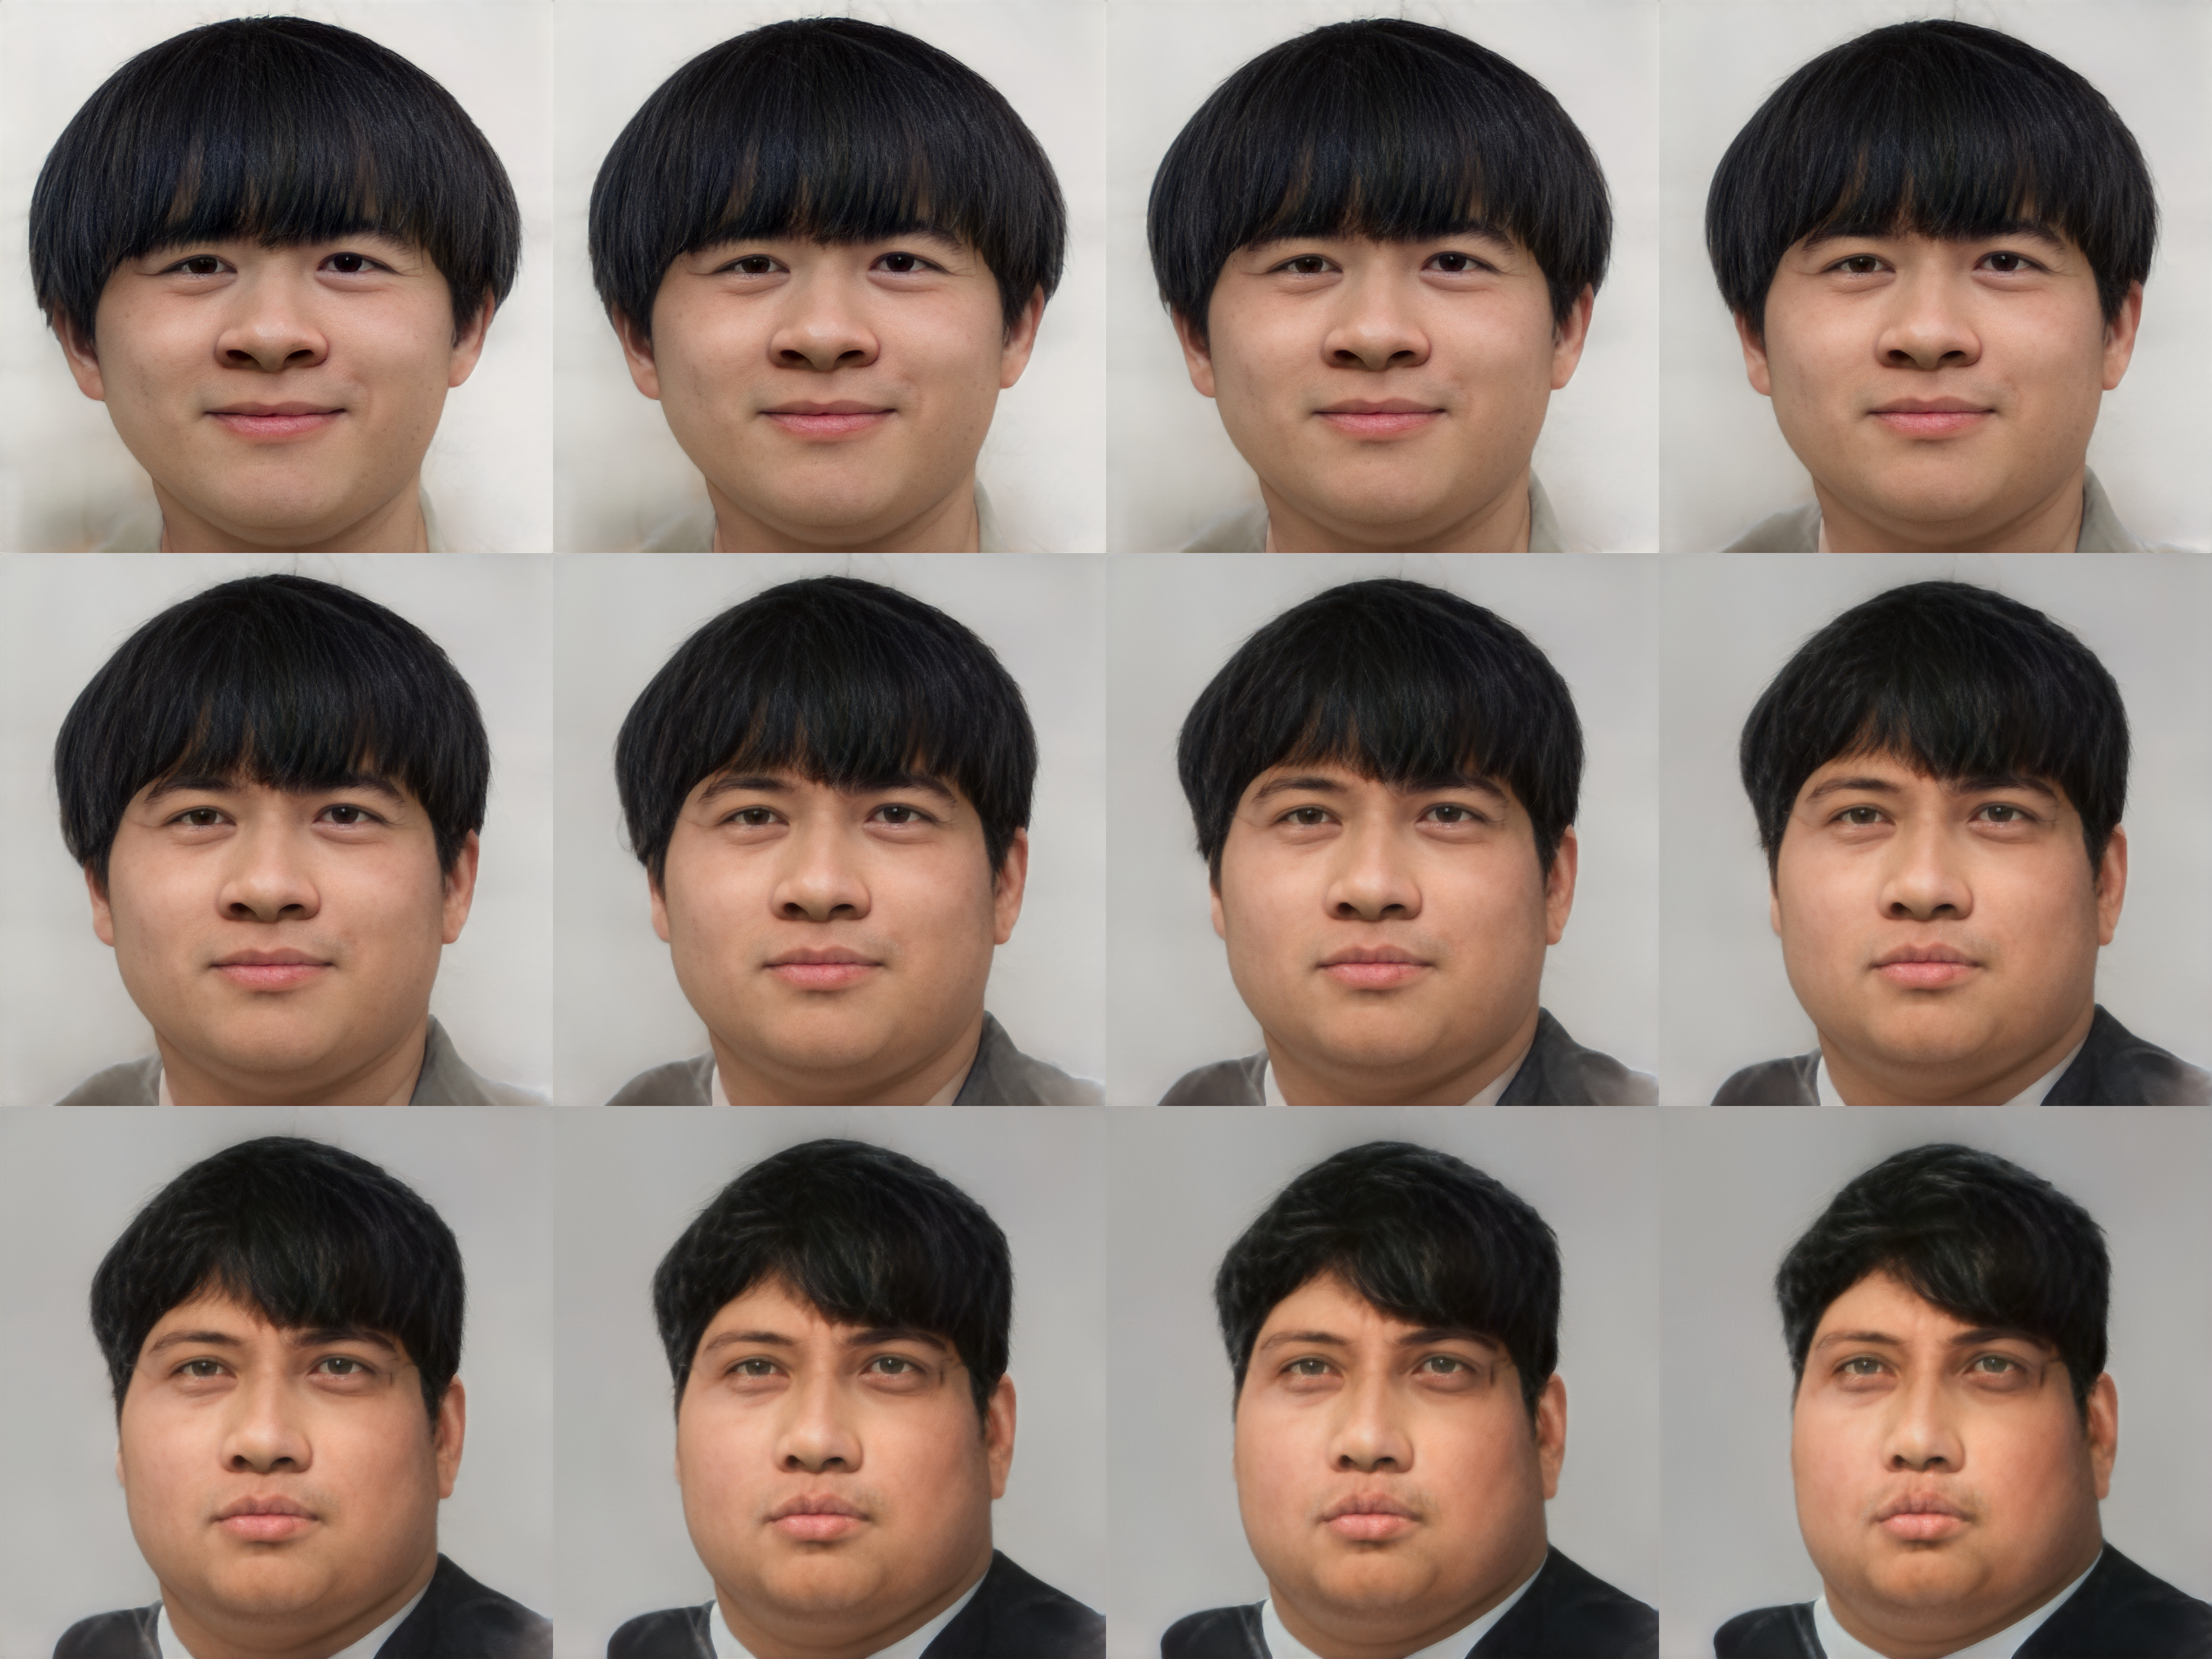
\includegraphics[scale=.05]{fig/change.png}
    \caption{Style fusion between source image and target image, upper left corner is the original reconstructed source image; while lower right corner is the original reconstructed target image}
    \label{fig:stylechange}
\end{figure}

\begin{figure}[ht]
\centering
    \centering
    \includegraphics[scale=.3]{fig/cmp_pair.png}
    \caption{face position problem}
    \label{fig:face position problem}
\end{figure}

\subsection{Human Pose Estimation}

The visualization result of human pose is shown in Figure \ref{fig:pose result}.

\begin{figure}[h]
\centering
    \centering
    \includegraphics[scale=.15]{fig/pose_result.png}
    \caption{pose result}
    \label{fig:pose result}
\end{figure}
\subsubsection{Implementation Detail}



We conduct an experiment on the accuracy of real-time human pose. There are left person and right person. Each action we do 10 times. 
\subsubsection{Evaluation Metric}
The result is shown in Table \ref{table:eval}. We got an excellent performance in hand raising hand and punching, which achieves 100\% accuracy. As for the last action "hands together", the accuracy is less than other. The main reason is that when we perform this action, the key point position of our hands will get very close, leading to self-occlusion. Under such condition, we observe that the prediction result of mediapipe becomes more unstable, so the average accuracy drops to 75\%.

\begin{table}
\begin{center}
\begin{tabular}{c|c|c|c|c}
\hline
Action & Test Case & \thead{Correct (L)} & \thead{Correct (R)} & \thead{Accuracy  (\%)}\\
\hline 
raise left hand & 10 & 10 & 10 & \textbf{100}\\
% \hline
raise right hand & 10 & 10 & 10& \textbf{100}\\
% \hline
punch left & 10 & 10 & 10 & \textbf{100}\\
% \hline
punch right & 10 & 10 & 10 & \textbf{100}\\
% \hline
hands together & 10 & 8 & 7 & 75 \\
\hline
\end{tabular}
\captionof{table}{Evaluation table for pose2action conversion. \texttt{correct (L)} and \texttt{correct (R)} stands for the number of correctly detected case for left person and right person in the game interface respectively.}
\label{table:eval}
\end{center}
\end{table}
% \begin{center}
% \begin{tabular}{c|c|c|c|c}
% \hline
% Action & test case & \thead{correct (L)} & \thead{correct (R)} & \thead{Accuracy  (\%)}\\
% \hline 
% raise left hand & 10 & 10 & 10 & \textbf{100}\\
% % \hline
% raise right hand & 10 & 10 & 10& \textbf{100}\\
% % \hline
% punch left & 10 & 10 & 10 & \textbf{100}\\
% % \hline
% punch right & 10 & 10 & 10 & \textbf{100}\\
% % \hline
% hands together & 10 & 8 & 7 & 75 \\
% \hline
% \end{tabular}
% \captionof{table}{Evaluation table for pose2action conversion. \texttt{correct (L)} and \texttt{correct (R)} stands for the number of correctly detected case for left person and right person in the game interface respectively.}
% \label{table:eval}
% \end{center}

\subsection{Game Interface}
After integrating with the human pose estimation and StyleGAN, we can use our body motions to control the game character and show the corresponding animation on the screen. Also, when the game character is being attacked, the face of the character will indeed change to the next style image. Finally, we have a live demo on the oral presentation, and the game is working perfectly from it starts to it ends.